\documentclass[12pt]{article}
\usepackage[utf8]{inputenc}
\usepackage{amsmath, amssymb, amsthm, graphicx, fancyvrb, enumitem, titlesec, setspace, float, fancyvrb, minted}
\usepackage[dvipsnames]{xcolor}
\usepackage[top=1in, bottom=1in, left=1.25in, right=1.25in]{geometry}
\titleformat{\section}{\normalfont\bfseries}{}{0em}{}
\titlespacing*{\section}{0pt}{1.5ex plus .2ex minus .2ex}{0.8ex plus .1ex}


\begin{document}
\noindent Andre Winkel \hfill \today \\
\rule{\textwidth}{0.4pt} \vspace{0em}
\begin{center} \large{Lab 5} \end{center} \vspace*{0em}

\section*{Problem 1: Plotting DTFS coefficients}
In this problem, we consider the periodic signal $x[n]$ with period $N$. Across its period,
\begin{equation}
    x[n]=
    \begin{cases}
        1 & \text{if } n\ge0 \text{ and } n<4.\\
        0 & \text{else.}
    \end{cases}
\end{equation}

\begin{enumerate}[label=\textbf{\alph*)}, leftmargin=2.6em]

\item We begin by computing the DTFS coefficients of this signal for $N=8$, and plot its magnitude and phase.

\begin{figure} [H]
    \centering
    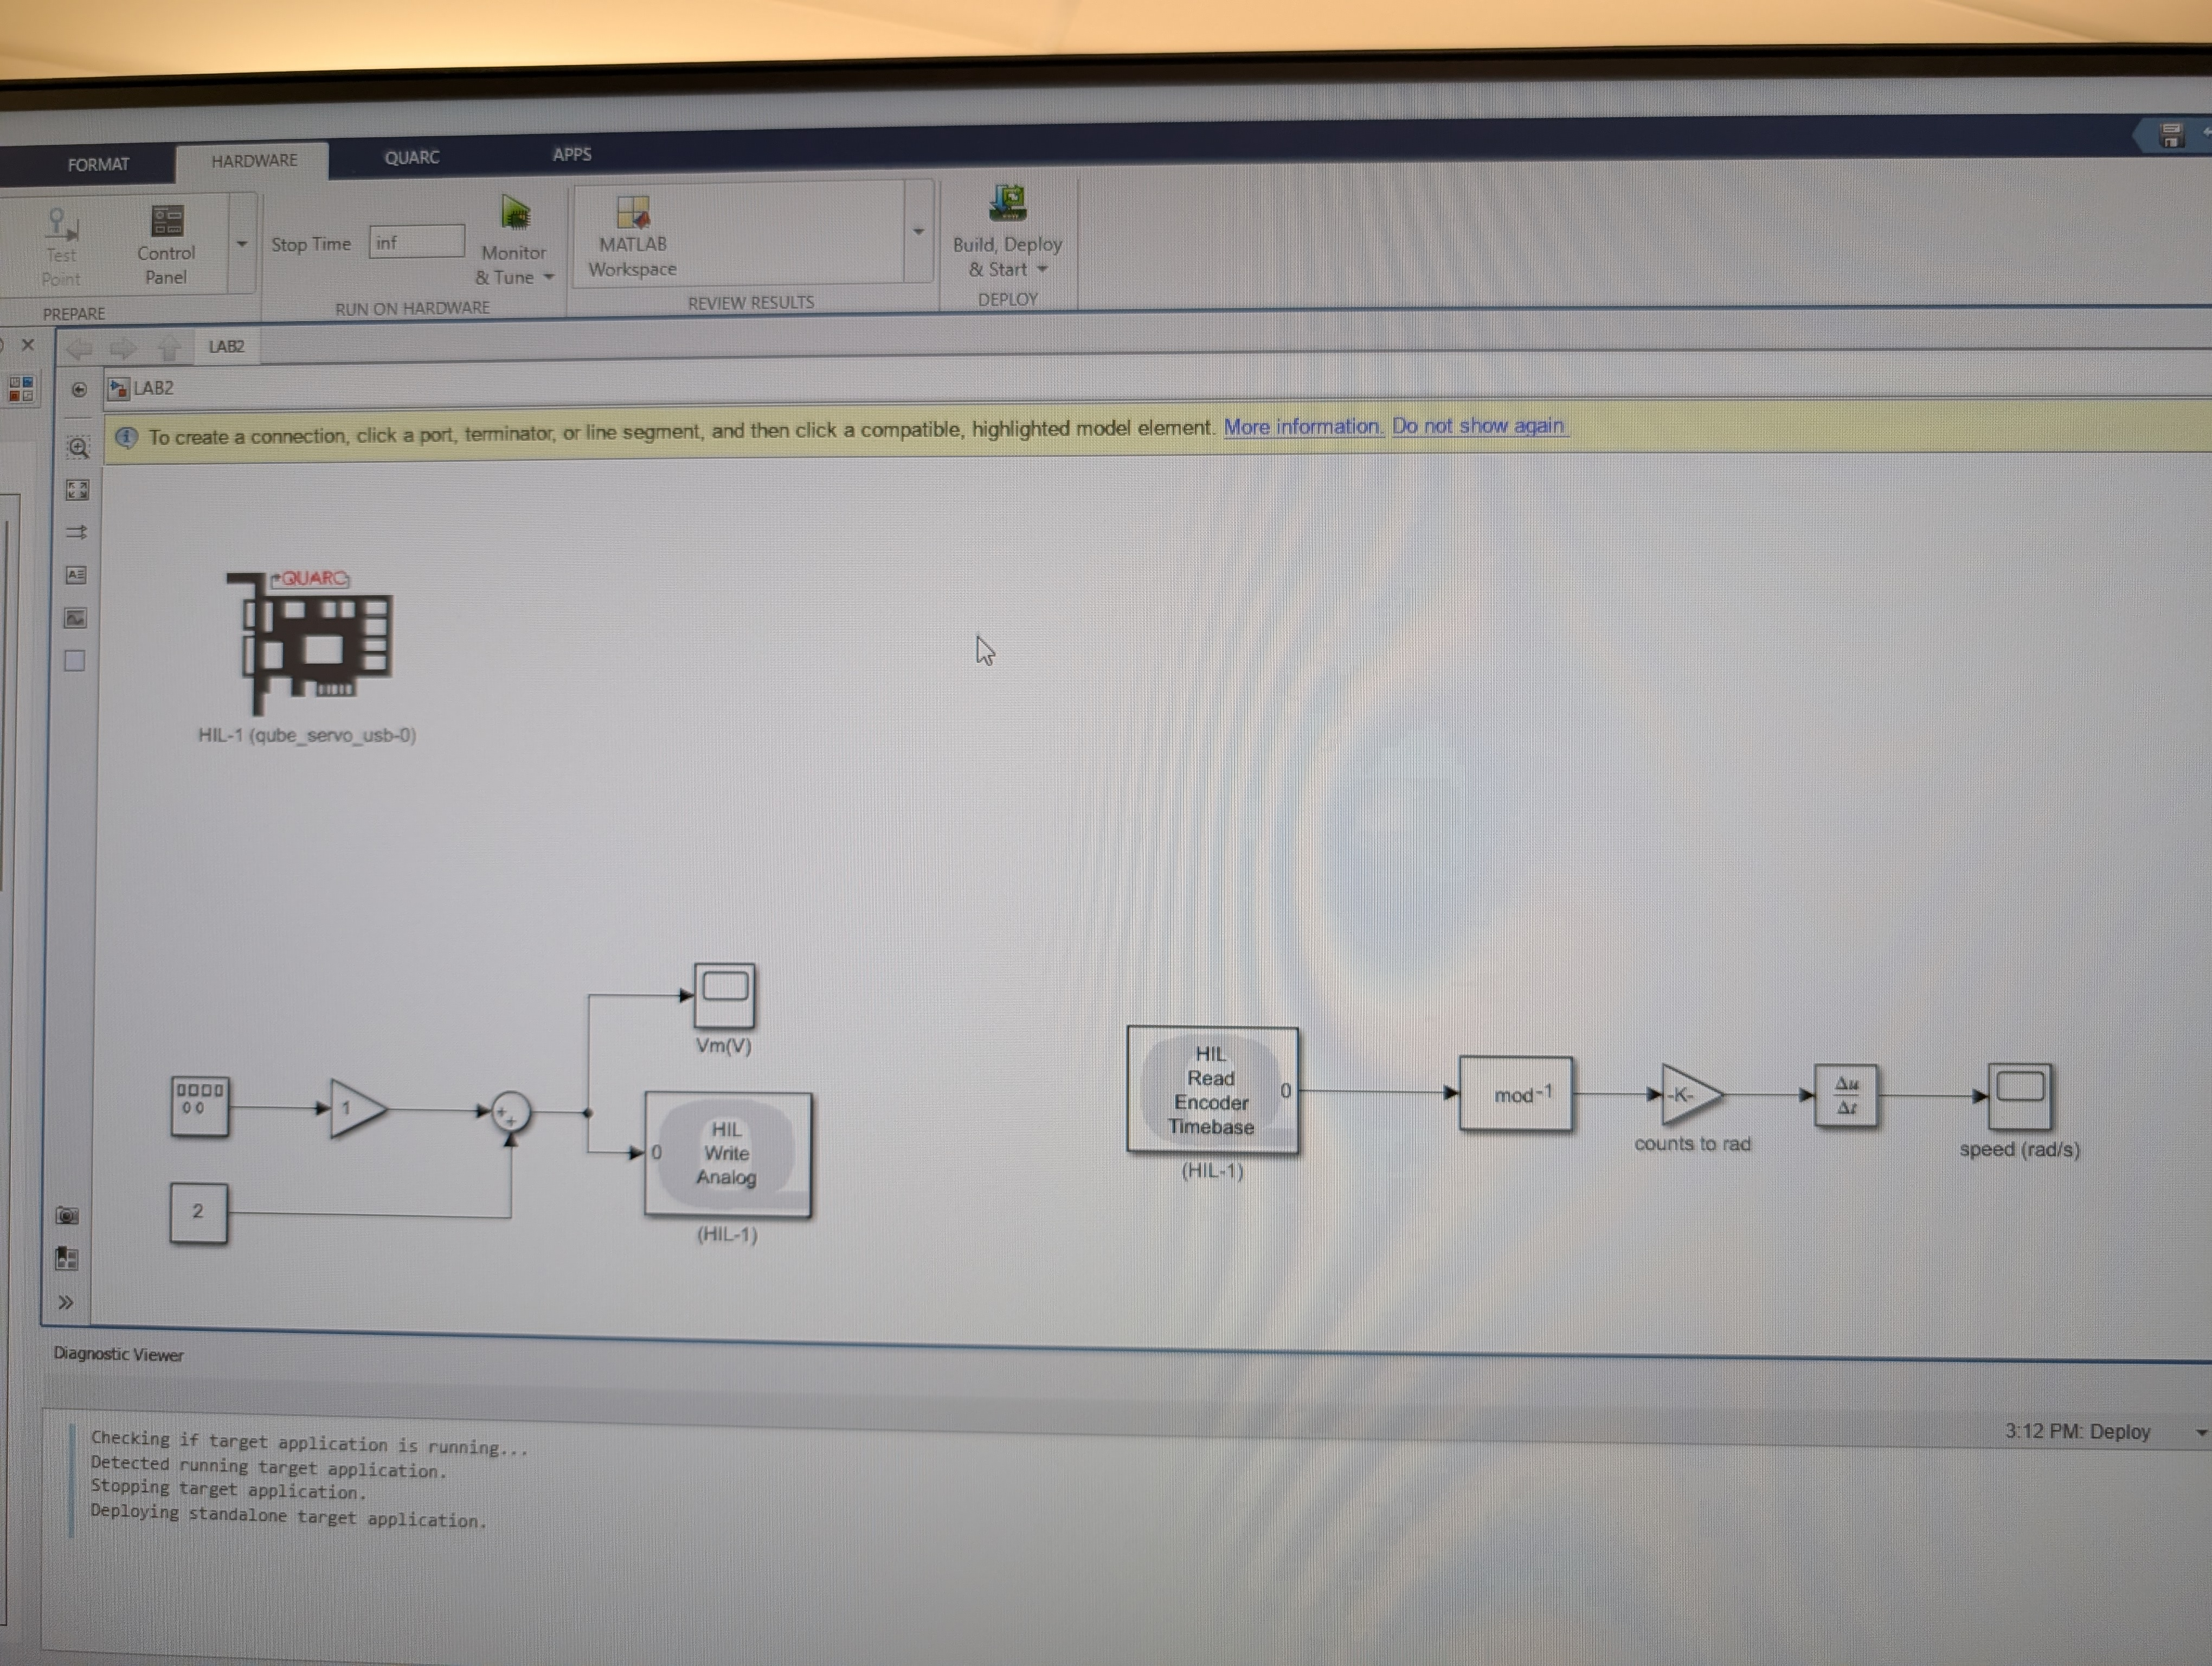
\includegraphics[width=0.4\linewidth]{1.png}
    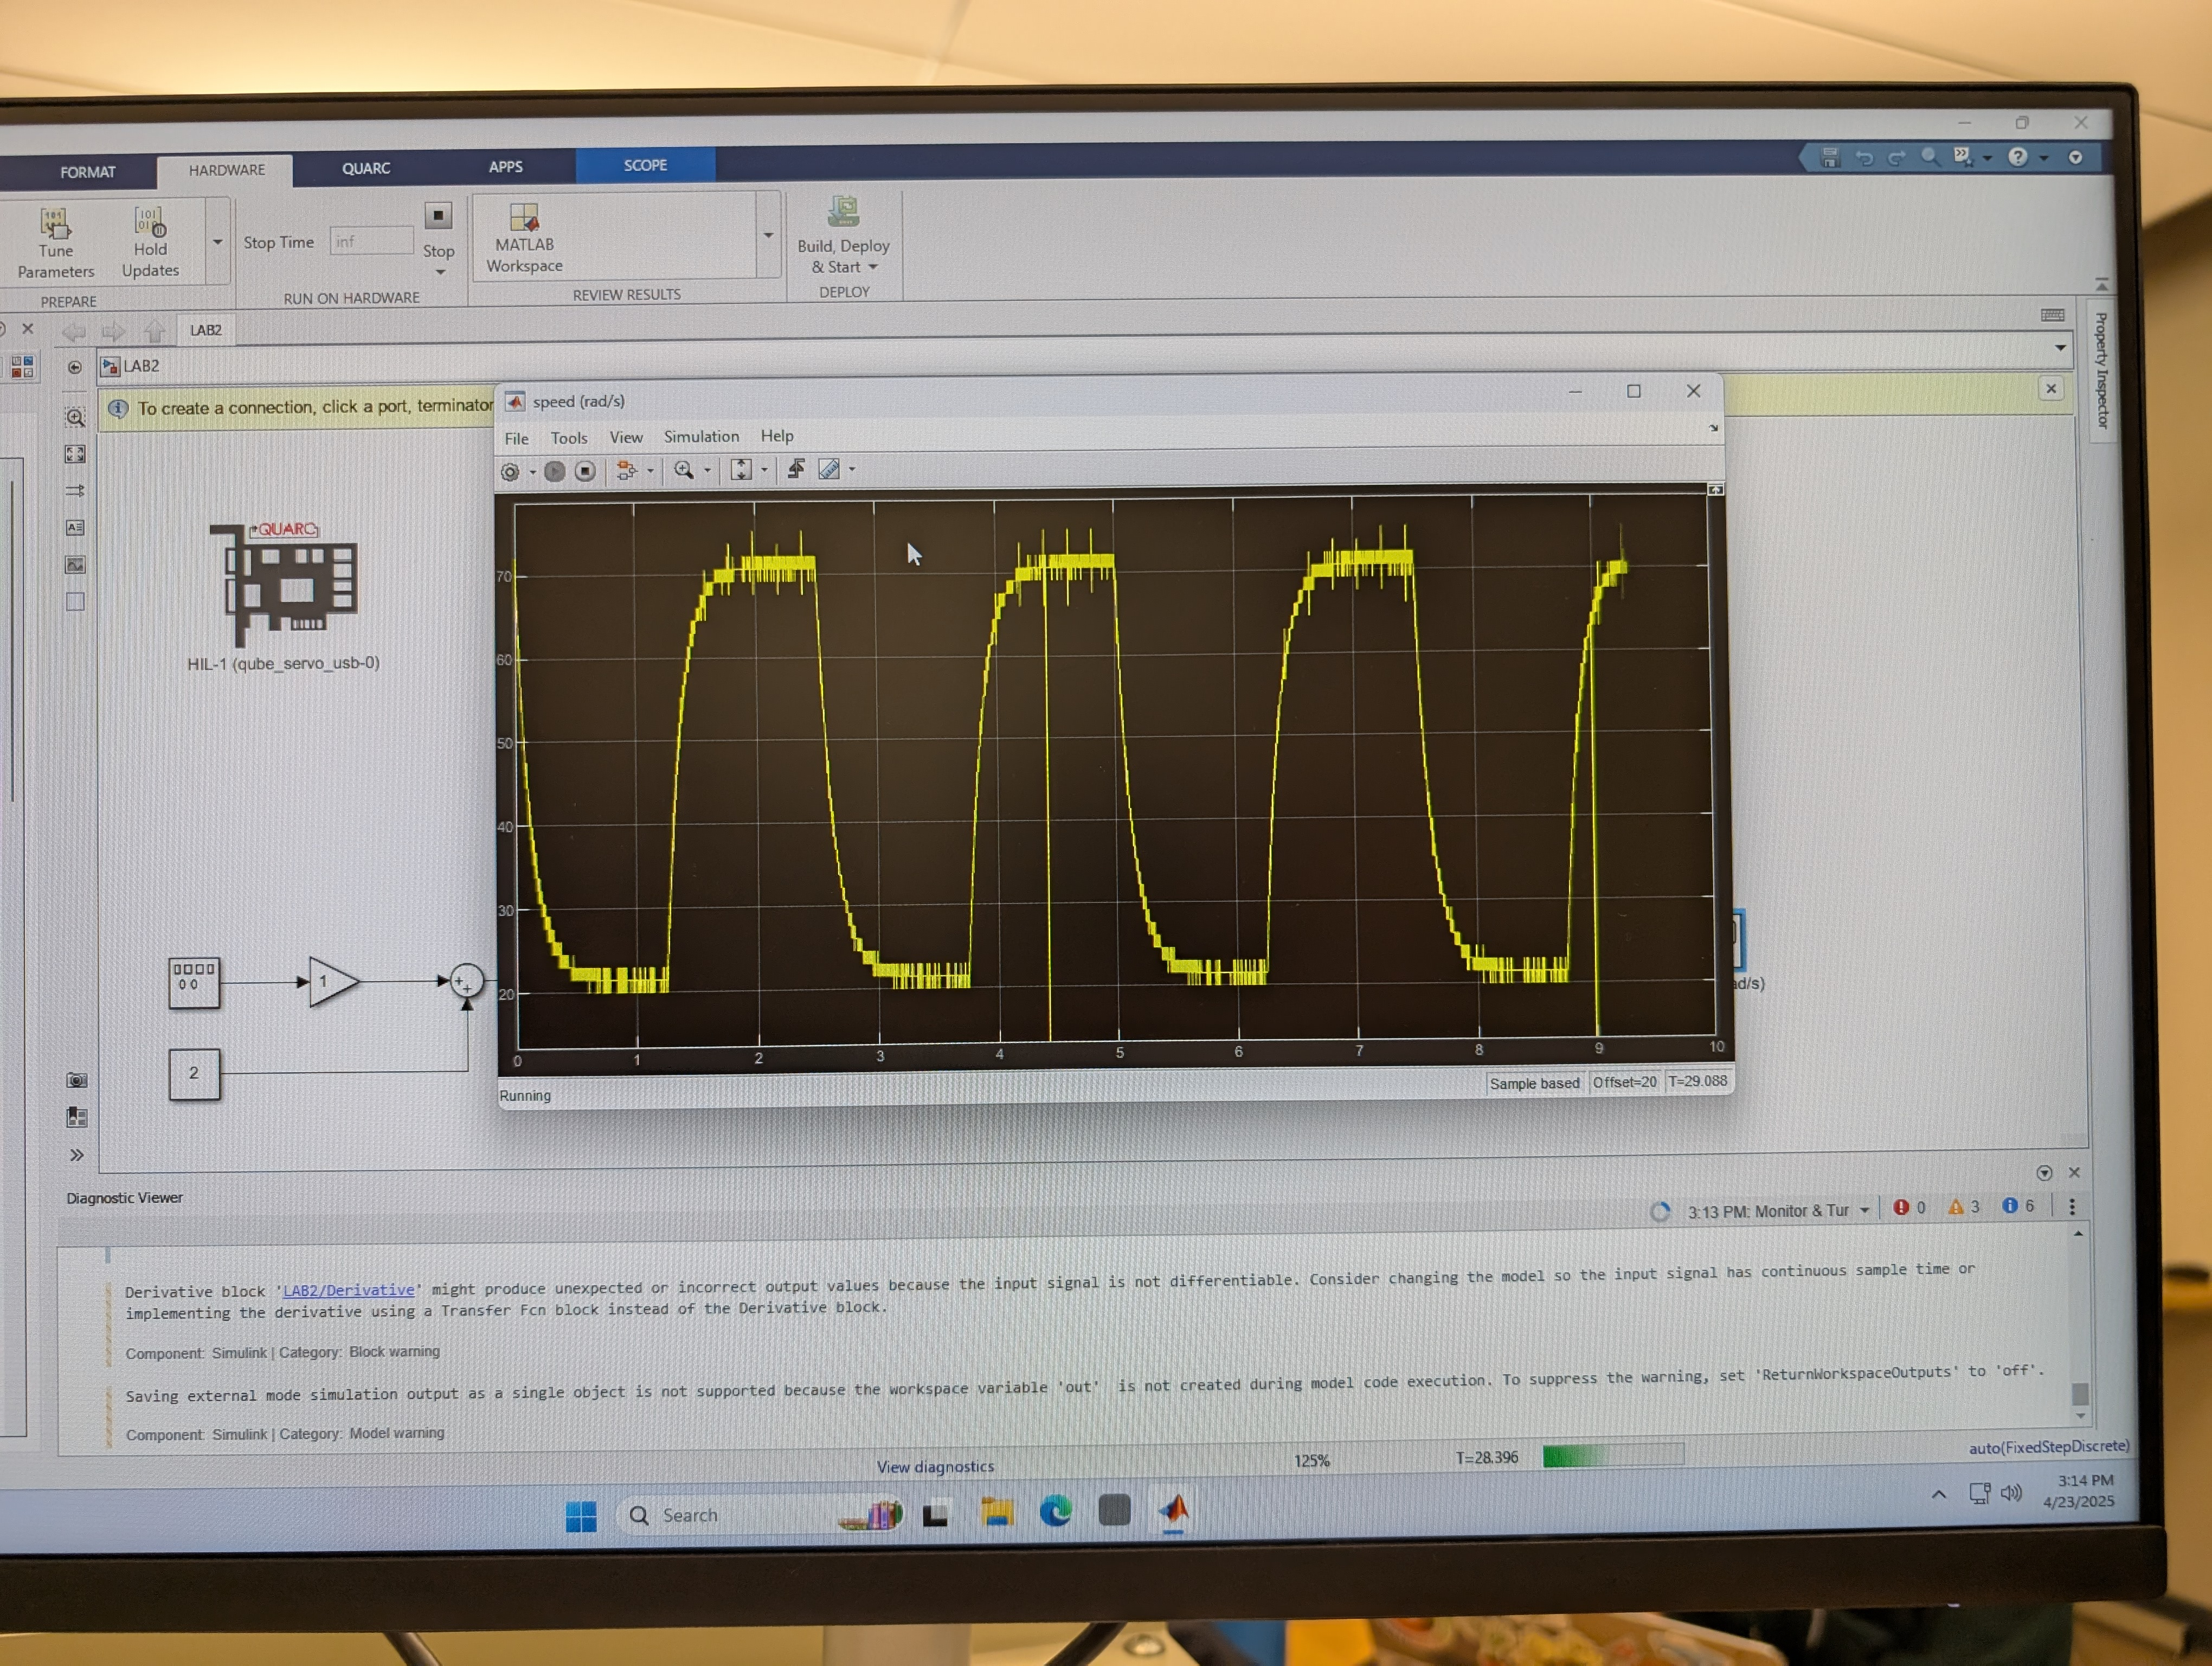
\includegraphics[width=0.4\linewidth]{2.png}
\end{figure}

\begin{minted}[frame=single, fontsize=\small, linenos, bgcolor=white]{matlab}
clear;
N = 8;
x_arr = zeros(1,N);

for idx = 1:N
    if idx < 4
        x_arr(idx)=1;
    end
end

x_dtfs = fft(x_arr);

dtfs_freqs = 2*pi*(0:(N-1))/N;

stem(dtfs_freqs, abs(x_dtfs), "filled", '.');
title('N=8 magnitude', 'FontSize', 16);
xlabel('\omega', 'FontSize', 16);
ylabel('|X[k]|', 'FontSize', 16);

stem(dtfs_freqs, angle(x_dtfs), "filled", '.');
title('N=8 phase', 'FontSize', 16);
xlabel('\omega', 'FontSize', 16);
ylabel('phase X[k]', 'FontSize', 16);
\end{minted}

\item We can then repeat part \textbf{a)} with $N=16$ and $N=256$, the plots of which being shown below:
\begin{figure}[H]
    \centering
    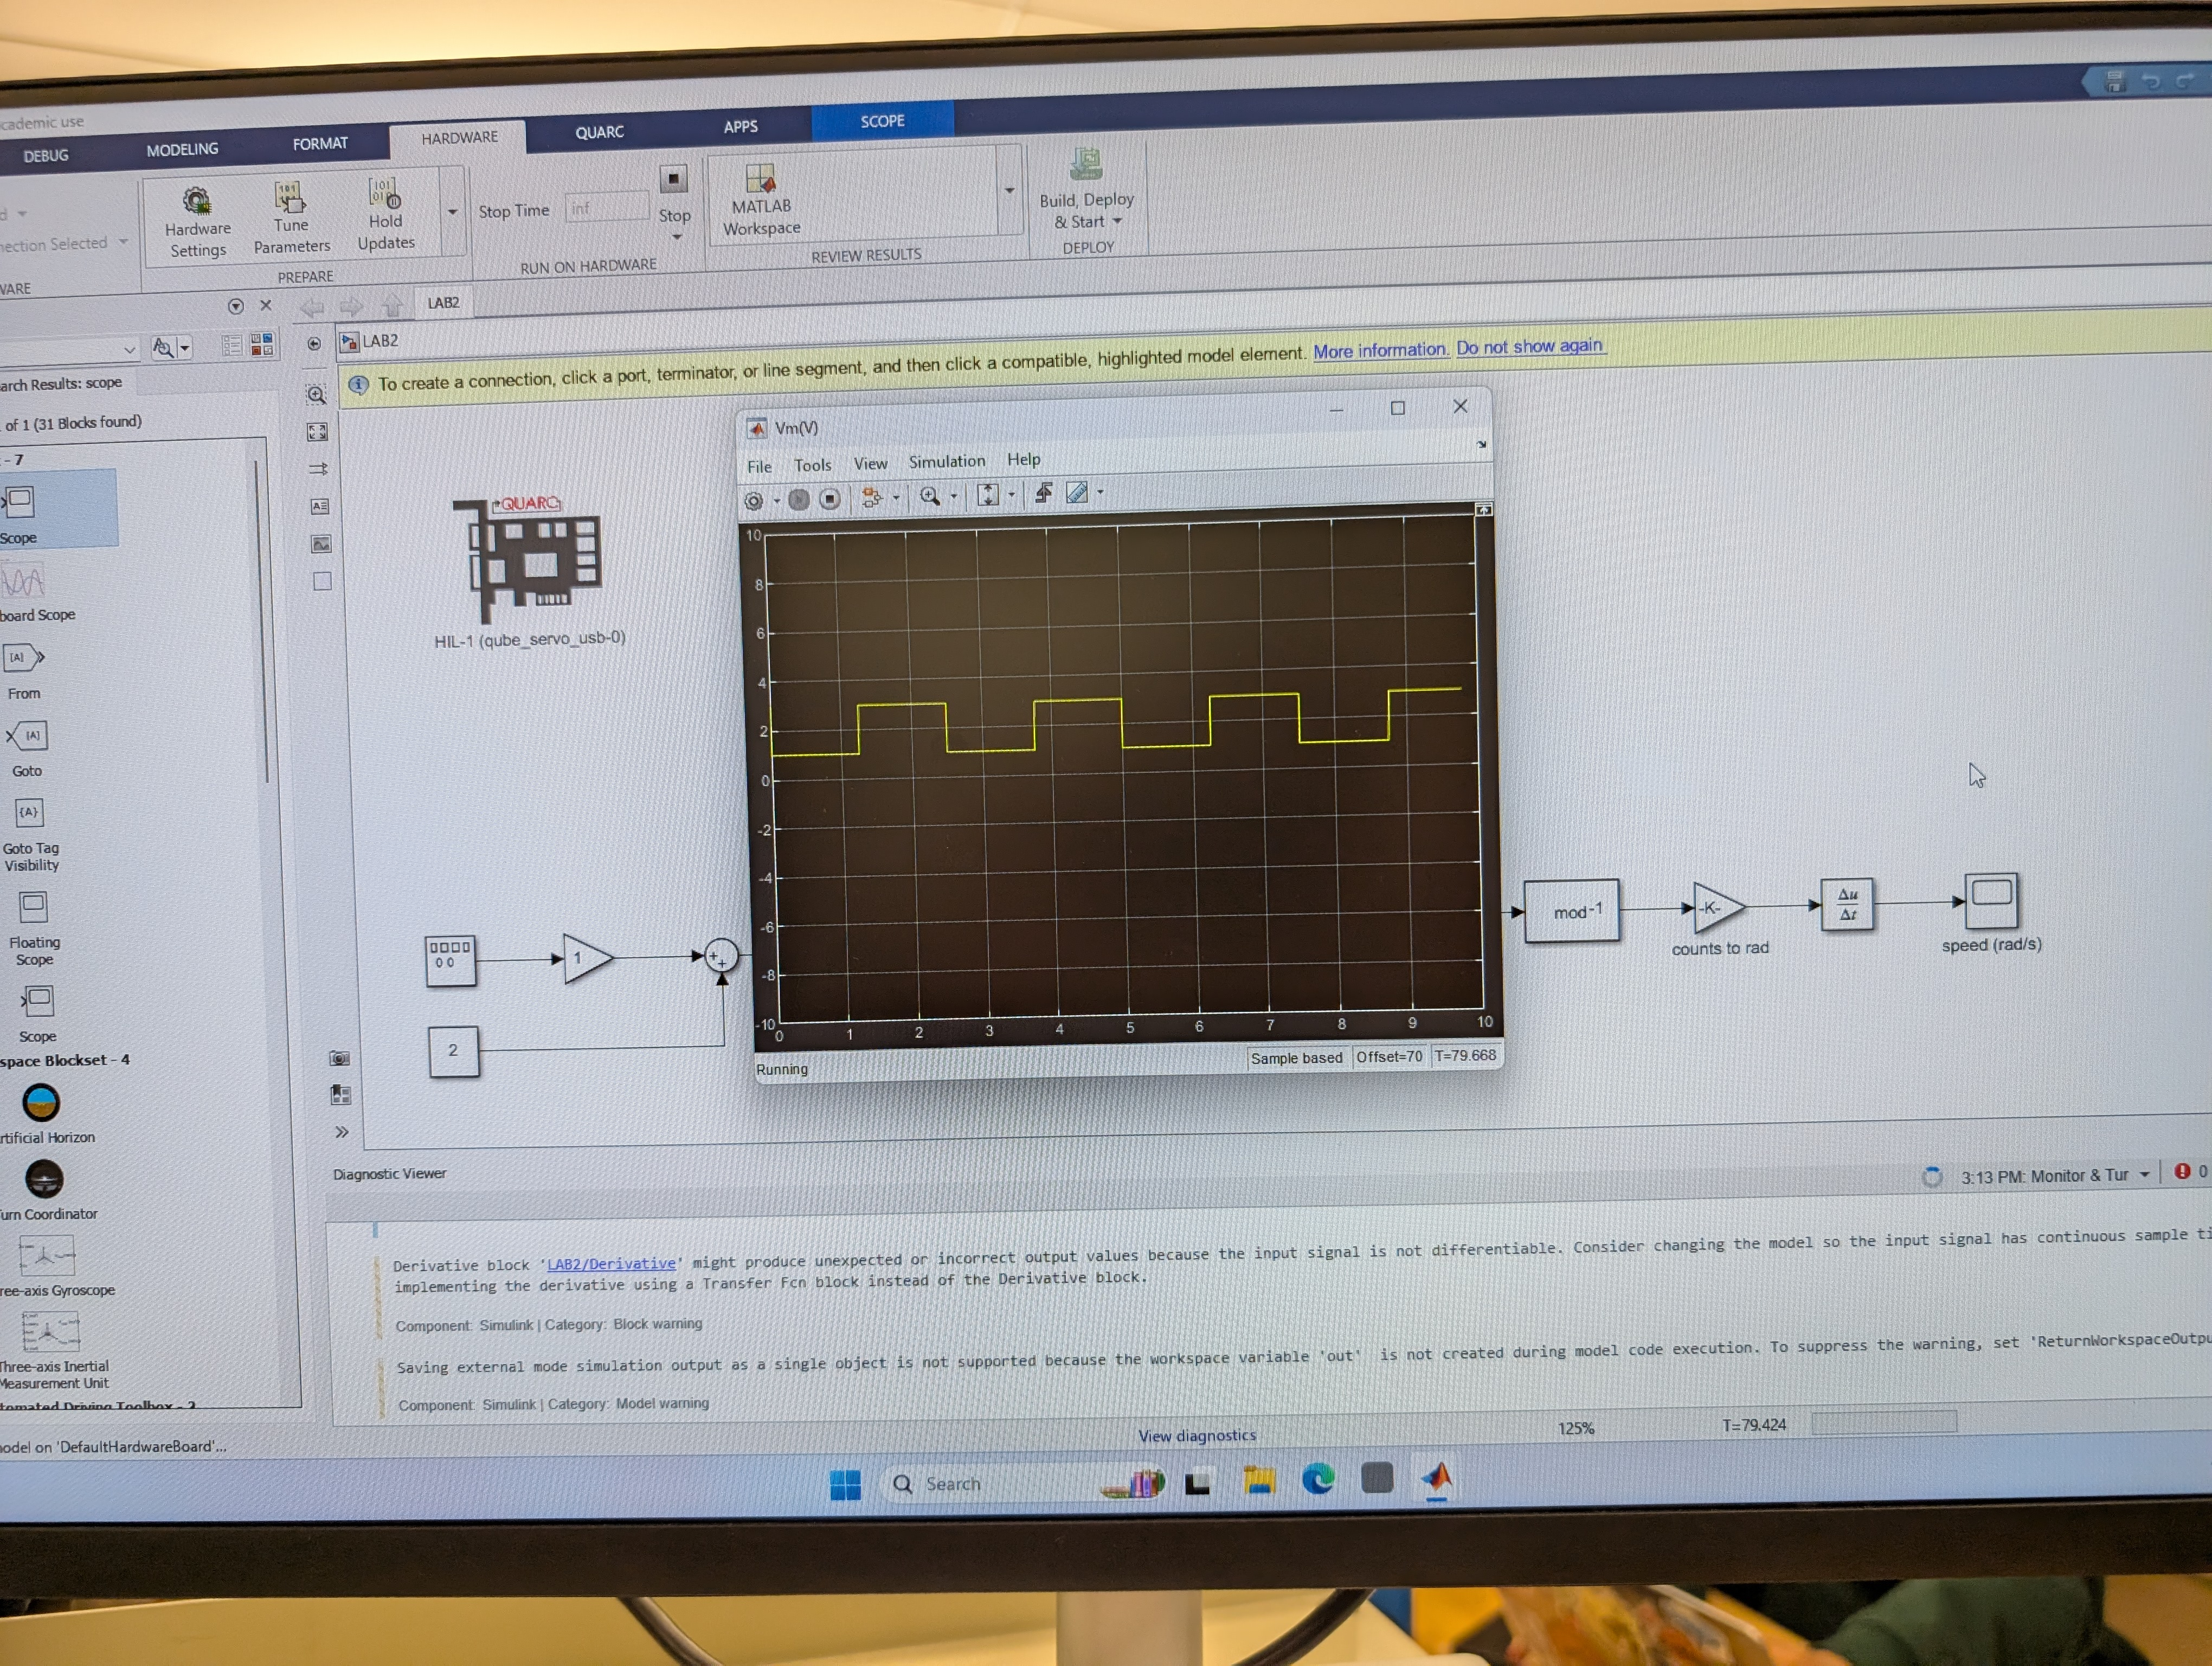
\includegraphics[width=0.4\linewidth]{3.png}
    \includegraphics[width=0.4\linewidth]{4.png}
\end{figure}
\begin{figure} [H]
    \centering
    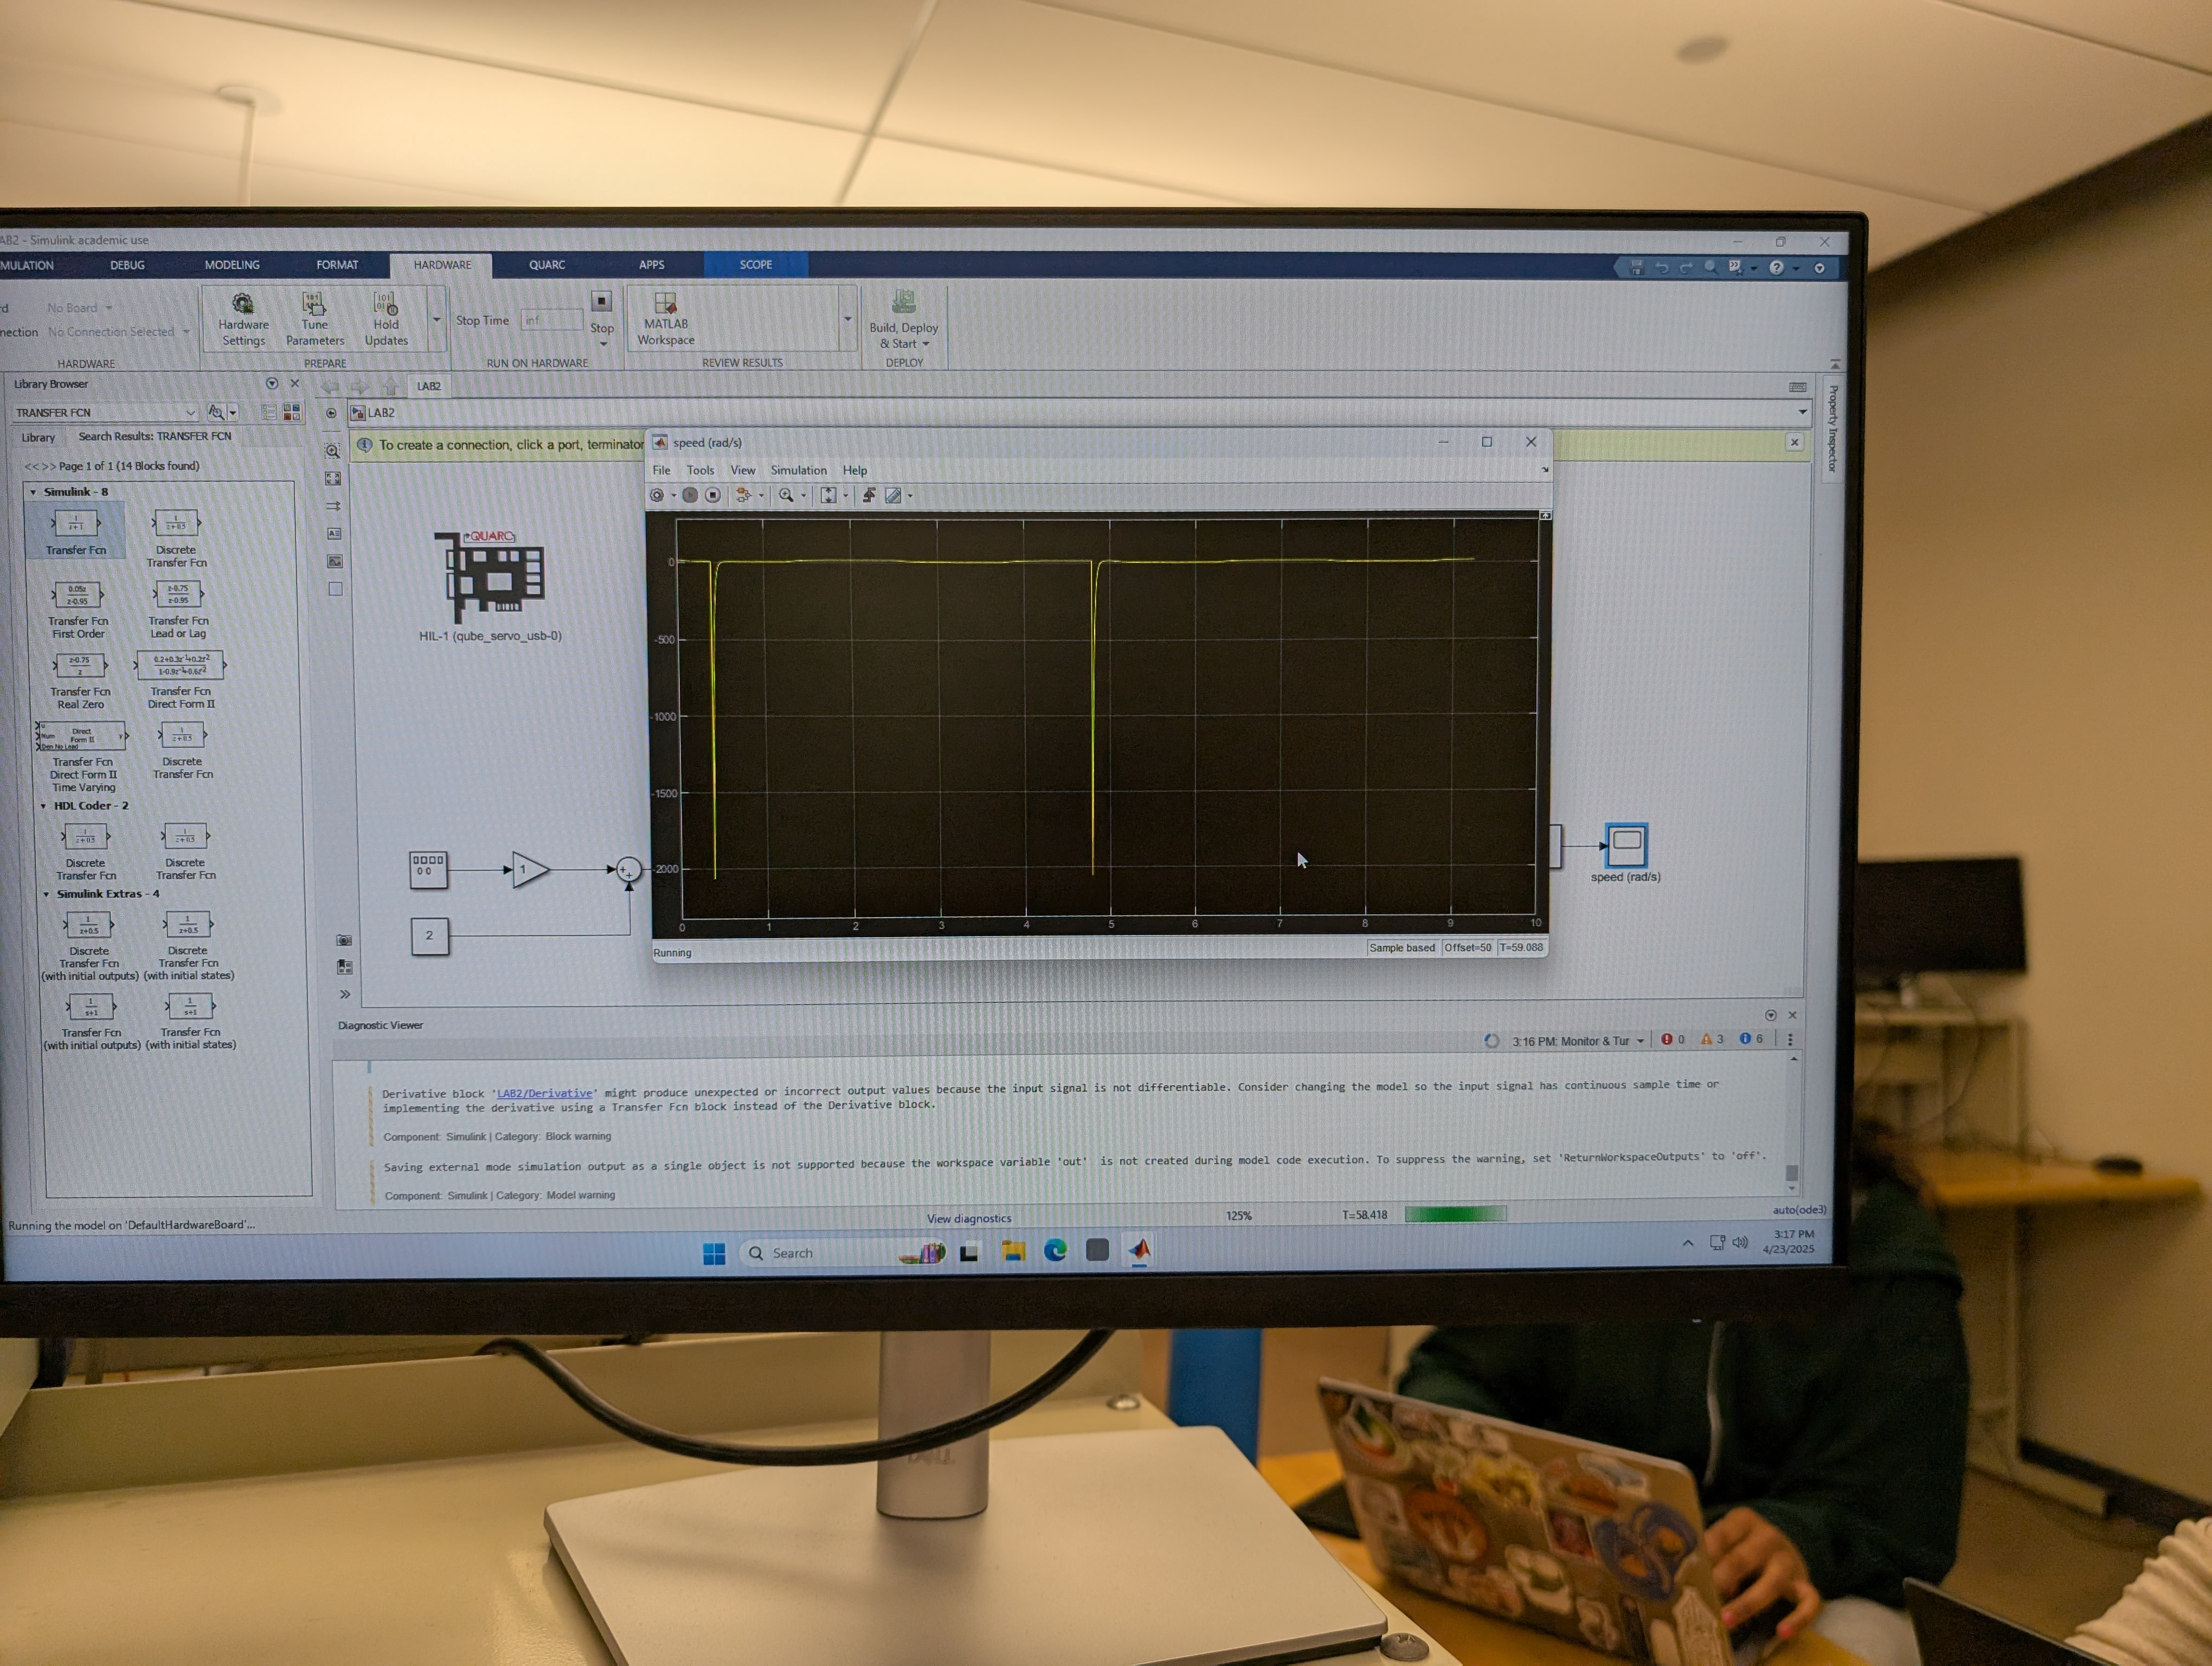
\includegraphics[width=0.4\linewidth]{5.png}
    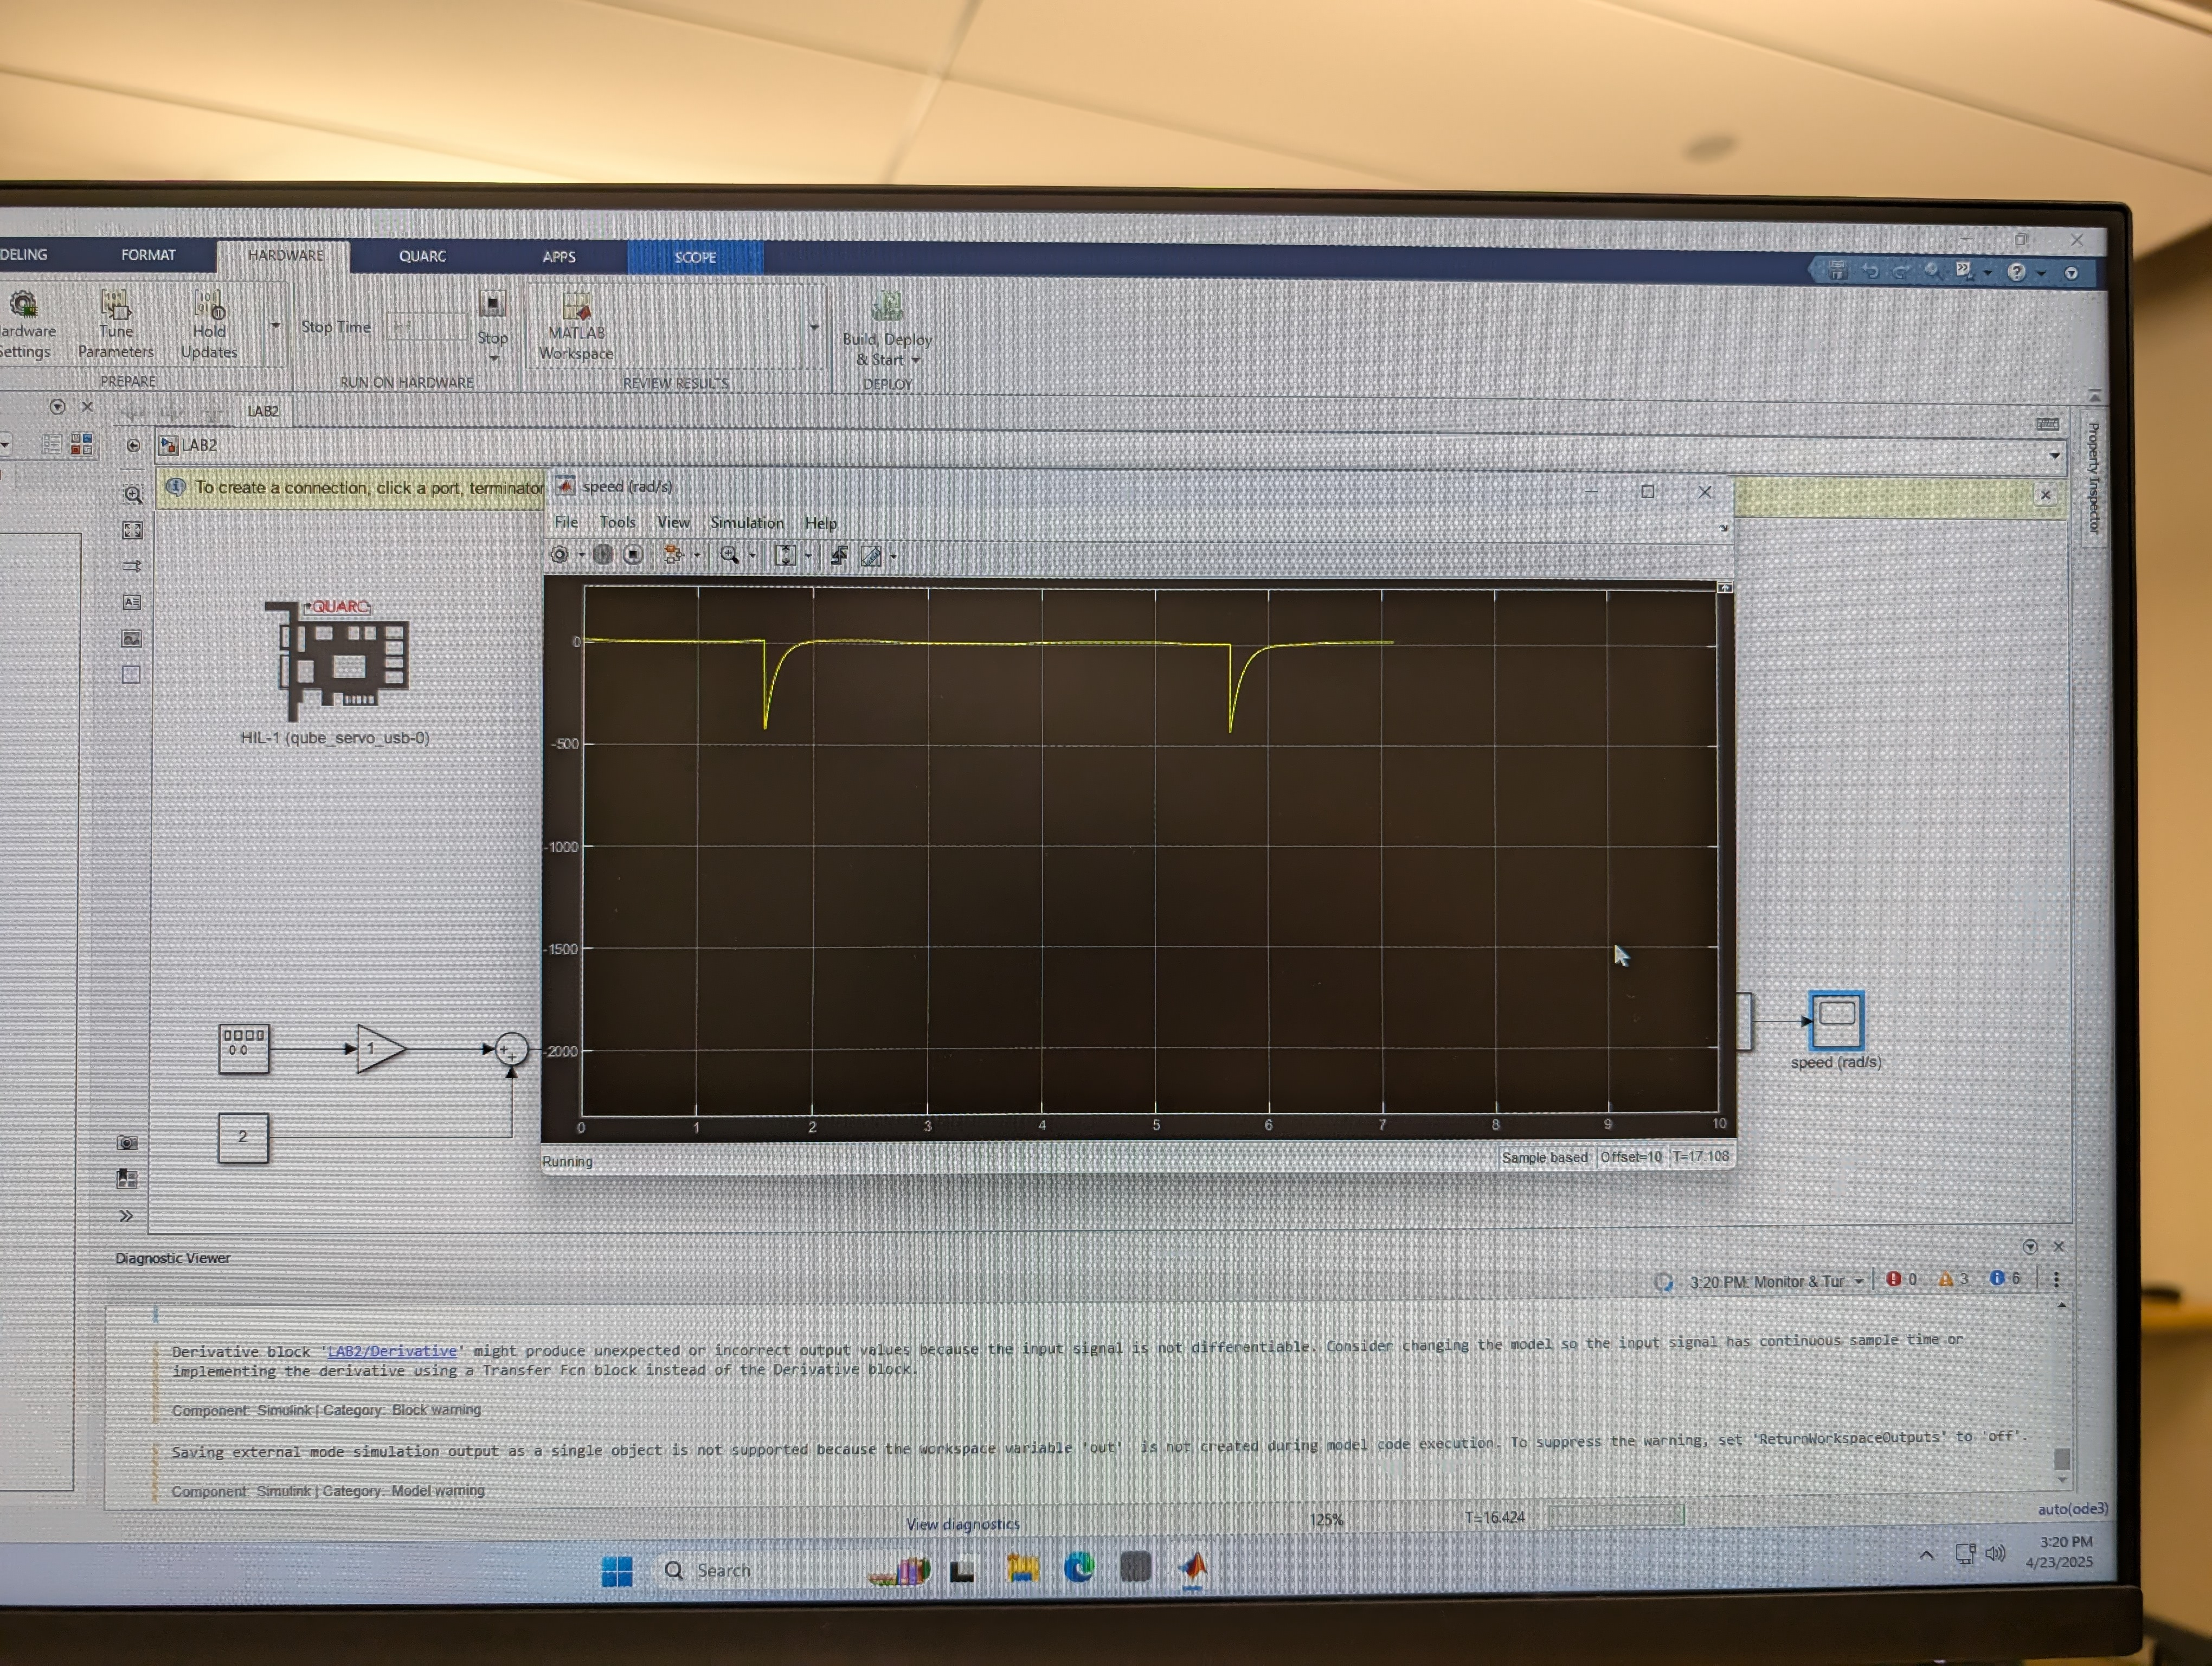
\includegraphics[width=0.4\linewidth]{6.png}
\end{figure}

\begin{minted}[frame=single, fontsize=\small, linenos, bgcolor=white]{matlab}
clear;
N = 256;
x_arr = zeros(1,N);

for idx = 1:N
    if idx < 4
        x_arr(idx)=1;
    end
end

x_dtfs = fft(x_arr);

dtfs_freqs = 2*pi*(0:(N-1))/N;

stem(dtfs_freqs, abs(x_dtfs), "filled", '.');
title('N=256 magnitude', 'FontSize', 16);
xlabel('\omega', 'FontSize', 16);
ylabel('|X[k]|', 'FontSize', 16);

stem(dtfs_freqs, angle(x_dtfs), "filled", '.');
title('N=256 phase', 'FontSize', 16);
xlabel('\omega', 'FontSize', 16);
ylabel('phase X[k]', 'FontSize', 16);
\end{minted}

We can then observe that as $N$ increases, both the magnitude and phase of the signal become clearer. It is seemingly important to notice that they all describe the same signal, however, only differing in resolution.

\end{enumerate}
\end{document}